% IEEE standard conference template; to be used with:
%   spconf.sty  - LaTeX style file, and
%   IEEEbib.bst - IEEE bibliography style file.
% --------------------------------------------------------------------------

\documentclass[letterpaper]{article}
\usepackage{spconf,amsmath,amssymb,graphicx}
\usepackage[utf8]{inputenc}
\usepackage{listings}
\usepackage{color}

\definecolor{dkgreen}{rgb}{0,0.6,0}
\definecolor{gray}{rgb}{0.5,0.5,0.5}
\definecolor{mauve}{rgb}{0.58,0,0.82}

\lstset{frame=tb,
  language=C++,
  aboveskip=3mm,
  belowskip=3mm,
  showstringspaces=false,
  columns=flexible,
  basicstyle={\small\ttfamily},
  numbers=none,
  numberstyle=\tiny\color{gray},
  keywordstyle=\color{blue},
  commentstyle=\color{dkgreen},
  stringstyle=\color{mauve},
  breaklines=true,
  breakatwhitespace=true
  tabsize=3
}

% Example definitions.
% --------------------
% nice symbols for real and complex numbers
\newcommand{\R}[0]{\mathbb{R}}
\newcommand{\C}[0]{\mathbb{C}}

% bold paragraph titles
\newcommand{\mypar}[1]{{\bf #1.}}

% Title.
% ------
\title{Optimization of the Metropolis Algorithm for a Potts Model}
%
% Single address.
% ---------------
\name{Dominik Gresch, Mario Könz\thanks{The author thanks Jelena Kovacevic. This paper
is a modified version of the template she used in her class.}} 
\address{Department of Physics\\ ETH Z\"urich\\Z\"urich, Switzerland}

% For example:
% ------------
%\address{School\\
%		 Department\\
%		 Address}
%
% Two addresses (uncomment and modify for two-address case).
% ----------------------------------------------------------
%\twoauthors
%  {A. Author-one, B. Author-two\sthanks{Thanks to XYZ agency for funding.}}
%		 {School A-B\\
%		 Department A-B\\
%		 Address A-B}
%  {C. Author-three, D. Author-four\sthanks{The fourth author performed the work
%		 while at ...}}
%		 {School C-D\\
%		 Department C-D\\
%		 Address C-D}
%

\begin{document}
%\ninept
%
\maketitle
%


\begin{abstract}
\end{abstract}

\section{Introduction}\label{sec:intro}

\mypar{Motivation} 
\mypar{Related work}

\section{Background: Potts Model and the Metropolis Algorithm}\label{sec:background}

\mypar{Potts Model}

\mypar{Metropolis Algorithm}

\mypar{Cost Analysis}


\section{Your Proposed Method}\label{sec:yourmethod}

\mypar{Autotuning}
\begin{lstlisting}
template<>
struct opt<150> {
    template<int S>
    using impl = greschd_v3_sim::impl<S, S, S, addon::mkl_mt_rng, msk_v1_pbc, msk_v2_dynamic_zip>; 
};

\end{lstlisting}

\begin{lstlisting}
template<int S, int N, bool B>
struct size_helper {
    static constexpr int size = size_helper<S, N - 1, S >= (sizes[N] + sizes[N - 1])/ 2 >::size;
};
\end{lstlisting}

\section{Experimental Results}\label{sec:exp}

\mypar{Experimental setup} 

\mypar{Results: SIM optimization}
	\begin{figure}[h]\centering
	  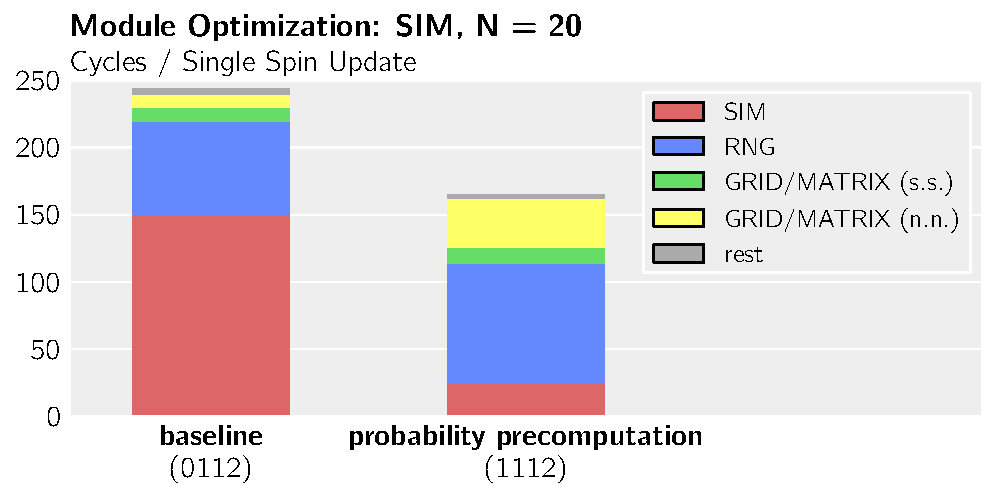
\includegraphics[width = 8.36cm]{plots/msk_20_2.pdf}
	  \caption{N = 20, SIM, Wolfdale}
	\end{figure}
	\begin{figure}[h]\centering
	  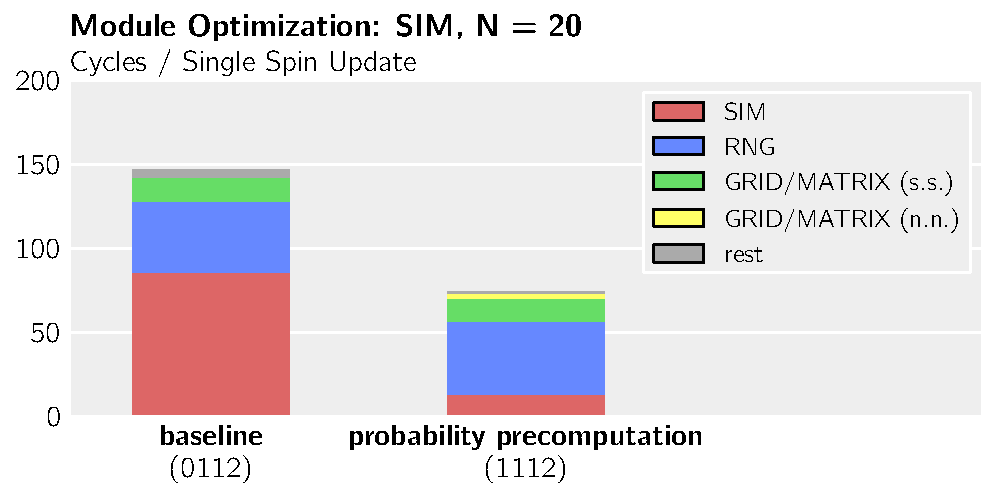
\includegraphics[width = 8.36cm]{plots/dg_20_2.pdf}
	  \caption{N = 20, SIM, Haswell}
	\end{figure}

\mypar{Results: GRID optimization}
	\begin{figure}[h]\centering
	  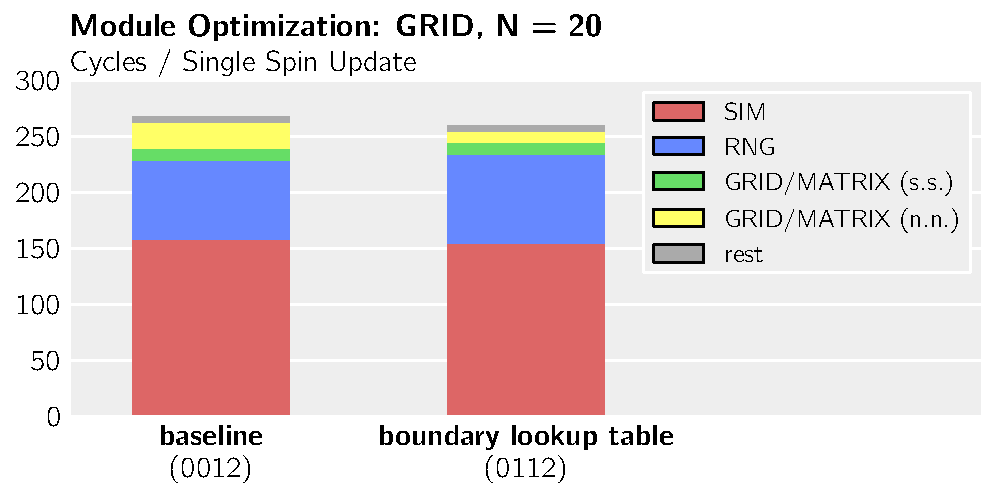
\includegraphics[width = 8.36cm]{plots/msk_20_1.pdf}
	  \caption{N = 20, GRID, Wolfdale}
	\end{figure}
	\begin{figure}[h]\centering
	  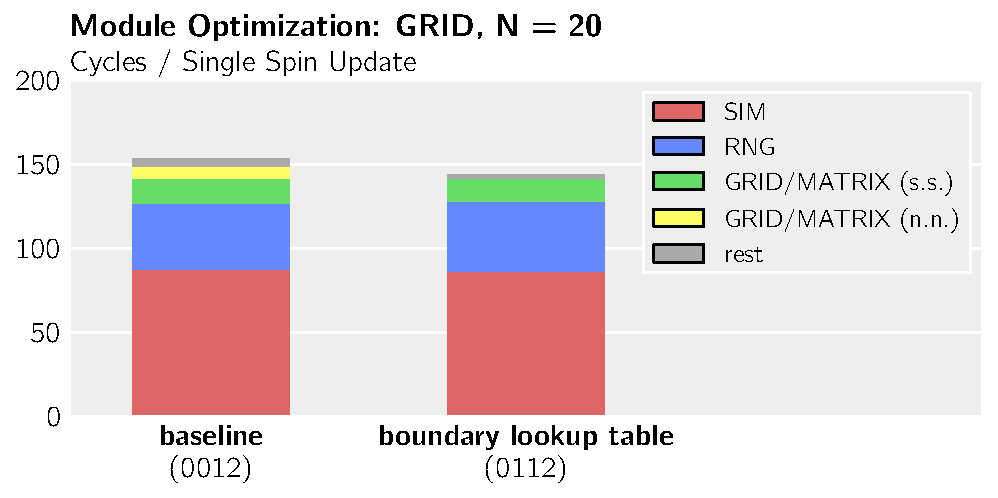
\includegraphics[width = 8.36cm]{plots/dg_20_1.pdf}
	  \caption{N = 20, GRID, Haswell}
	\end{figure}

\mypar{Results: MATRIX optimization}
	\begin{figure}[h]\centering
	  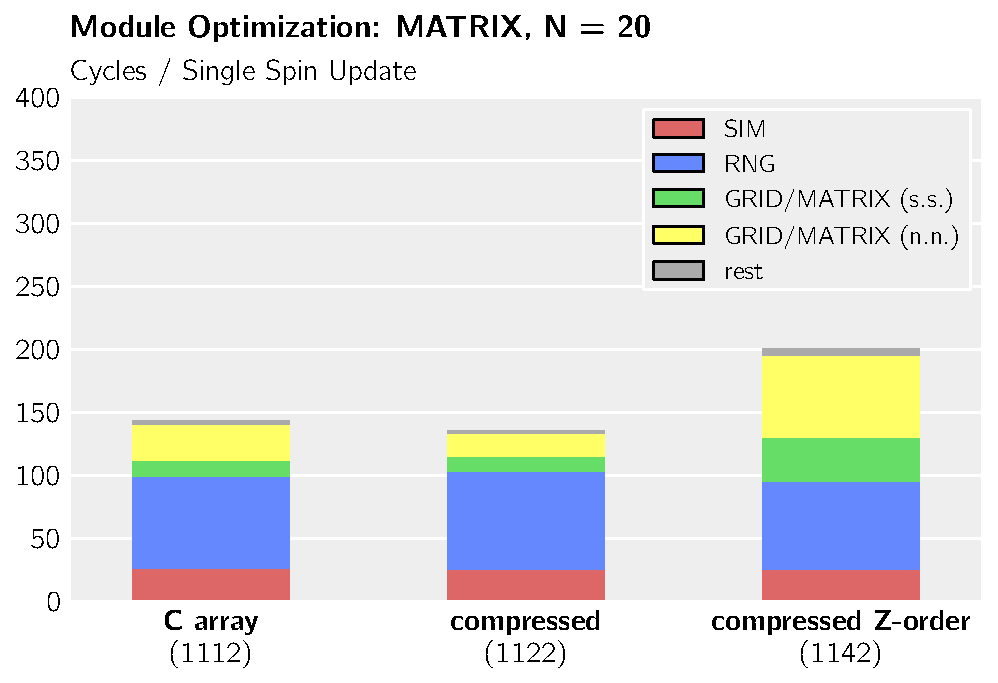
\includegraphics[width = 8.36cm]{plots/msk_20_3.pdf}
	  \caption{N = 20, MATRIX, Wolfdale}
	\end{figure}
	
	\begin{figure}[h]\centering
	  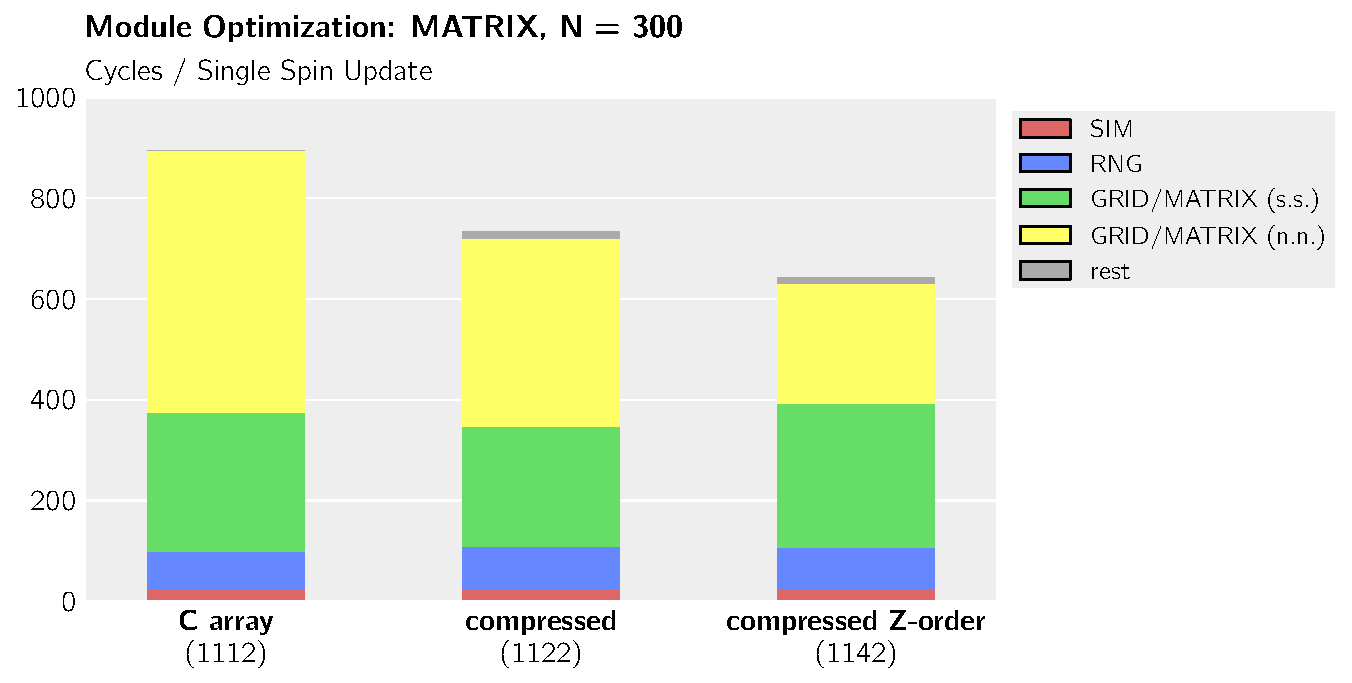
\includegraphics[width = 8.36cm]{plots/msk_300_3.pdf}
	  \caption{N = 300, MATRIX, Wolfdale}
	\end{figure}
	
	\begin{figure}[h]\centering
	  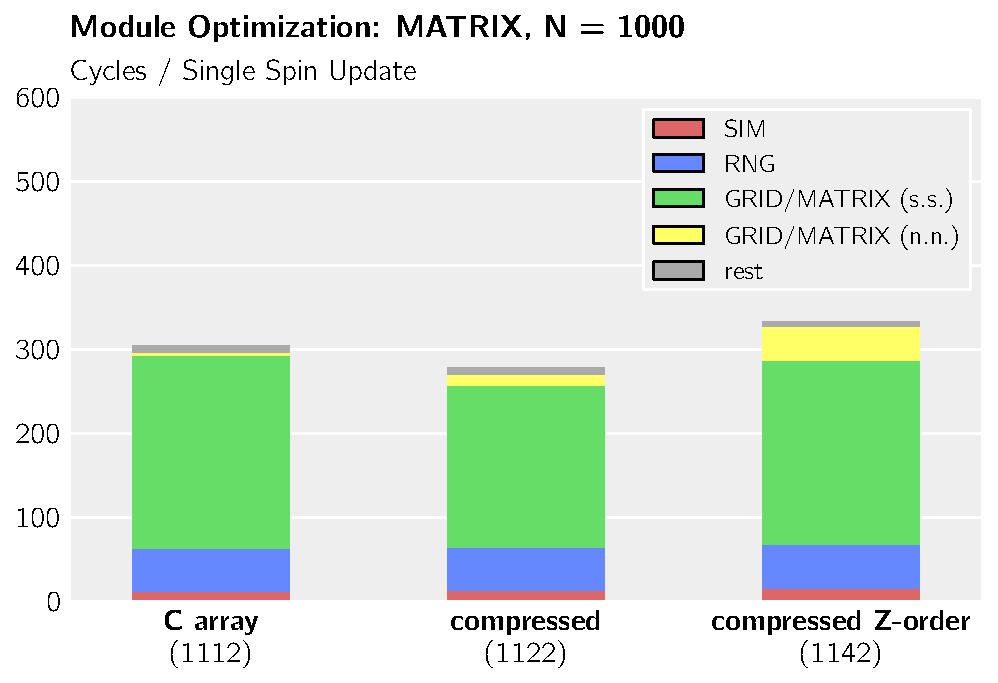
\includegraphics[width = 8.36cm]{plots/dg_1000_3.pdf}
	  \caption{N = 1000, MATRIX, Haswell}
	\end{figure}
\mypar{Results: RNG optimization}
	\begin{figure}[h]\centering
	  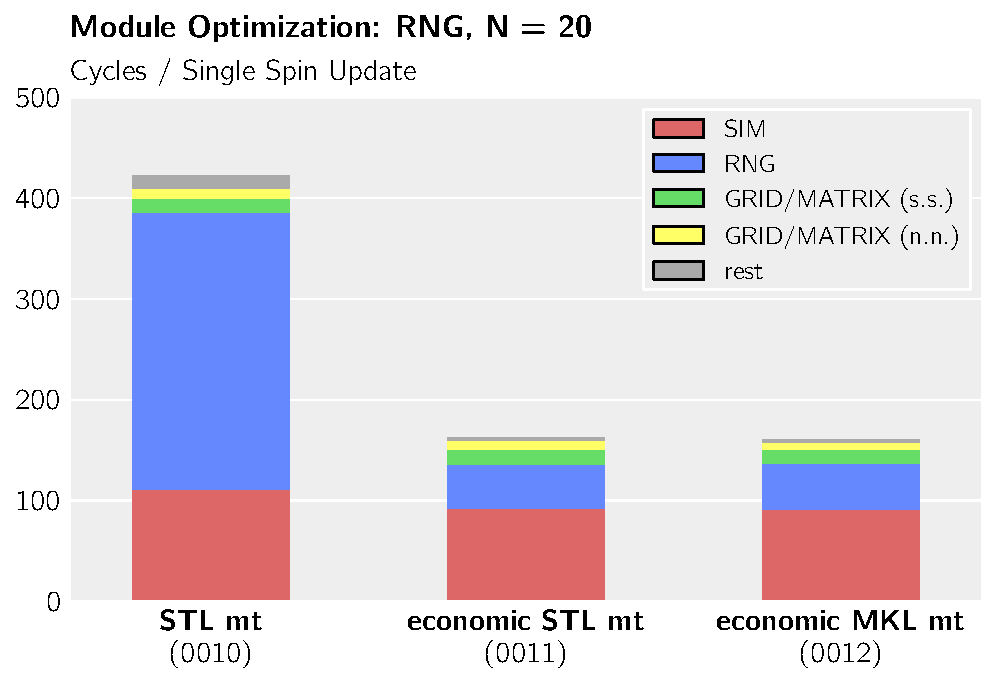
\includegraphics[width = 8.36cm]{plots/dg_20_0.pdf}
	  \caption{N = 20, RNG, Haswell}
	\end{figure}

\mypar{Results: Autotuning}

\mypar{Results: Performance}

\section{Conclusions}


\section{Further comments}
\bibliography{bibl_conf}

\end{document}

